\IEEEraisesectionheading{\section{正交变换}
\label{sec:orthogonal_transformation}}

 \lettrine{数}{字}图像处理的方法主要分为两大类,一个是空间域处理法(或称空域法),一个是频域法(或称变换域法)。在频域法中最为关键的预处理便是变换处理,这种变换一般是线性变换。具体而言,就是将空域中的信号(图像)变换到另外一个域(频域),即使用该域中的一组单位正交基函数(相同基函数内积为1,不同基函数内积为0)的线性组合来表示任意函数。使用这组基函数的线性组合得到任意函数$f$,每个基函数的系数就是$f$与该基函数的内积。

图像变换通常是一种二维正交变换,一般要求必须是可逆的,正变换和反变换的算法不能太复杂,而且在变换域中图像能量将集中分布在低频率成分上,边缘、线状信息反映在高频率成分上。这样做可以使图像处理问题简化,有利于图像特征提取并有助于从概念上增强对图像信息的理解。因此,正交变换被广泛地运用于图像特征提取、图像增强、图像复原、图像识别以及图像编码等处理中。主要的正交变换包括傅立叶变换、离散余弦变换、沃尔什变换、哈尔变换、斜变换和小波变换。

傅里叶变换是大家所熟知的正交变换,在一维信号处理中有着广泛应用。把这种处理方法推广到图像处理中是很自然的事。通俗来讲,一维傅立叶变换是将一个一维的信号分解成若干个复指数波$e^{jwx}$。而由于$e^{jwx} =cos(wx)+jsin(wx)$,所以可以将每一个复指数波$e^{jwx}$都视为是余弦波 $+ j\times$ 正弦波的组合。一维信号是一个序列,傅立叶变换将其分解成若干个一维的简单函数之和。二维信号可以说是一个图像,类比一维,那二维傅立叶变换就是将图像分解成基图像(即复平面波$e^{ji\pi (ux+vy)}$)之和,这些基图像是相互正交的,图像变换的本质是寻找合适的基图像来表达图像。

		对图像进行二维傅里叶变换得到的频谱图,中心部分表示原图像中的低频部分,是图像中灰度变化不太快的成分,反映了图像的主体框架;频谱的四周,也即是高频区域是图像中灰度变化较快的成分,一般反映着图像中的椒盐噪声(突发性的白点或黑点)或者是图像内部变化剧烈的边缘成分。
	
	傅里叶变换的一个最大问题是它的参数都是复数,在数据的描述上相当于实数的两倍。而离散余弦变换为全实数的正交变换,能够达到和傅立叶变换相同功能但数据量又不大。二维离散余弦变换的定义由下式表示:
	
\begin{equation}
\begin{aligned}
& F(0,0)=\frac{1}{N} \sum_{x=0}^{N-1} \sum_{y=0}^{N-1} f(x, y) \\
& F(0, v)=\frac{\sqrt{2}}{N} \sum_{x=0}^{N-1} \sum_{y=0}^{N-1} f(x, y) \cdot \cos \frac{(2 y+1) v \pi}{2 N} \\
& F(u, 0)=\frac{\sqrt{2}}{N} \sum_{x=0}^{N-1} \sum_{y=0}^{N-1} f(x, y) \cos \frac{(2 x+1) u \pi}{2 N} \\
& F(u, v)=\frac{2}{N} \sum_{x=0}^{N-1} \sum_{y=0}^{N-1} f(x, y) \cos \frac{(2 x+1) u \pi}{2 N} \cdot \cos \frac{(2 y+1) v \pi}{2 N}
\end{aligned}
\end{equation}

二维离散余弦反变换的定义由下式表示:

\begin{equation}
\begin{aligned}
f(x, y) & =\frac{1}{N} F(0,0)+\frac{\sqrt{2}}{N} \sum_{v=1}^{N-1} F(0, v) \cos \frac{(2 y+1) v \pi}{2 N} \\
& +\frac{\sqrt{2}}{N} \sum_{u=1}^{N-1} F(u, 0) \cos \frac{(2 x+1) u \pi}{2 N} \\
& +\frac{2}{N} \sum_{u=1}^{N-1} \sum_{v=1}^{N-1} F(u, v) \cos \frac{(2 x+1) u \pi}{2 N} \cdot \cos \frac{(2 y+1) v \pi}{2 N}
\end{aligned}
\end{equation}

与傅里叶变换一样,离散余弦变换自然可以由定义 式出发进行计算。但这样的计算量太大,在实际应 用中很不方便。所以也要寻求一种快速算法。 首先,从定义出发,作如下推导:

\begin{equation}
\begin{aligned}
F(u) & =\sqrt{\frac{2}{N}} \sum_{x=0}^{N-1} f(x) \cos \frac{(2 x+1) u \pi}{2 N} \\
& =\sqrt{\frac{2}{N}} \sum_{x=0}^{N-1} f(x) R_e\left\{e^{-j \frac{(2 x+1) u \pi}{2 N}}\right\} \\
& =\sqrt{\frac{2}{N}} R_e\left\{\sum_{x=0}^{N-1} f(x) e^{-j \frac{(2 x+1) u \pi}{2 N}}\right\}
\end{aligned}
\vspace{0.3cm}
\end{equation}

如果把时域数据数据向量作下列延拓,即:

\begin{equation}
f_e(x)= \begin{cases}f(x) & x=0,1,2, \cdots \cdots, N-1 \\ 0 & x=N, N+1, \cdots \cdots, 2 N-1\end{cases}
\vspace{0.3cm}
\end{equation}

则 $f_e(x)$ 的离散余弦变换可写作下式:

\begin{equation}
\begin{aligned}
F(0) & =\frac{1}{\sqrt{N}} \sum_{x=0}^{2 N-1} f_e(x) \\
F(u) & =\sqrt{\frac{2}{N}} \sum_{x=0}^{2 N-1} f_e(x) \cos \frac{(2 x+1) u \pi}{2 N} \\
& =\sqrt{\frac{2}{N}} R_e\left\{\sum_{x=0}^{2 N-1} f_e(x) e^{-j \frac{(2 x+1) u \pi}{2 N}}\right\} \\
& =\sqrt{\frac{2}{N}} R_e\left\{e^{-j \frac{u \pi}{2 N}} \cdot \sum_{x=0}^{2 N-1} f_e(x) e^{-j \frac{2 x u \pi}{2 N}}\right\}
\end{aligned}
\vspace{0.3cm}
\end{equation}

可见 $\sum_{x=0}^{2 N-1} f_e(x) e^{-j \frac{2 x u \pi}{2 N}}$ 正是延拓后 $2N$ 点的离散傅立叶变换。所以在作离散余弦变换时,可以把序列长度延拓为 $2N$,然后作离散傅里叶变换,产生的结果取其实部便可得到余弦变换。同样,离散余弦反变换可以从 $\left[F_e(u) \cdot e^{j \frac{u \pi}{2 N}}\right]$ 的 $2N$ 点反傅立叶变换实现。

\begin{figure}[!ht]
	\centering
	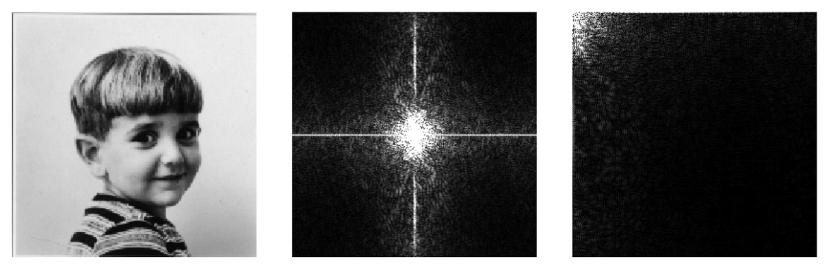
\includegraphics[width=\linewidth]{1.png}
	\caption{原始图像及快速傅立叶变换、离散余弦变换频谱图}
	\label{fig:fig1}
\end{figure}

如 \textbf{图 \ref{fig:fig1}} 所示,除了数据存储量和运算速度的差别,在变换获得的频谱图方面,离散傅立叶变换也比傅立叶变换更加集中。具体运用方面,离散余弦变换是JPEG有损压缩算法的基础(JPEG2000是基于小波变换的图像压缩标准,压缩比更高,而且不会产生基于离散余弦变换的JPEG标准产生的分块效应)。其算法流程如 \textbf{图 \ref{fig:fig2}} 所示。

\begin{figure}[!ht]
	\centering
	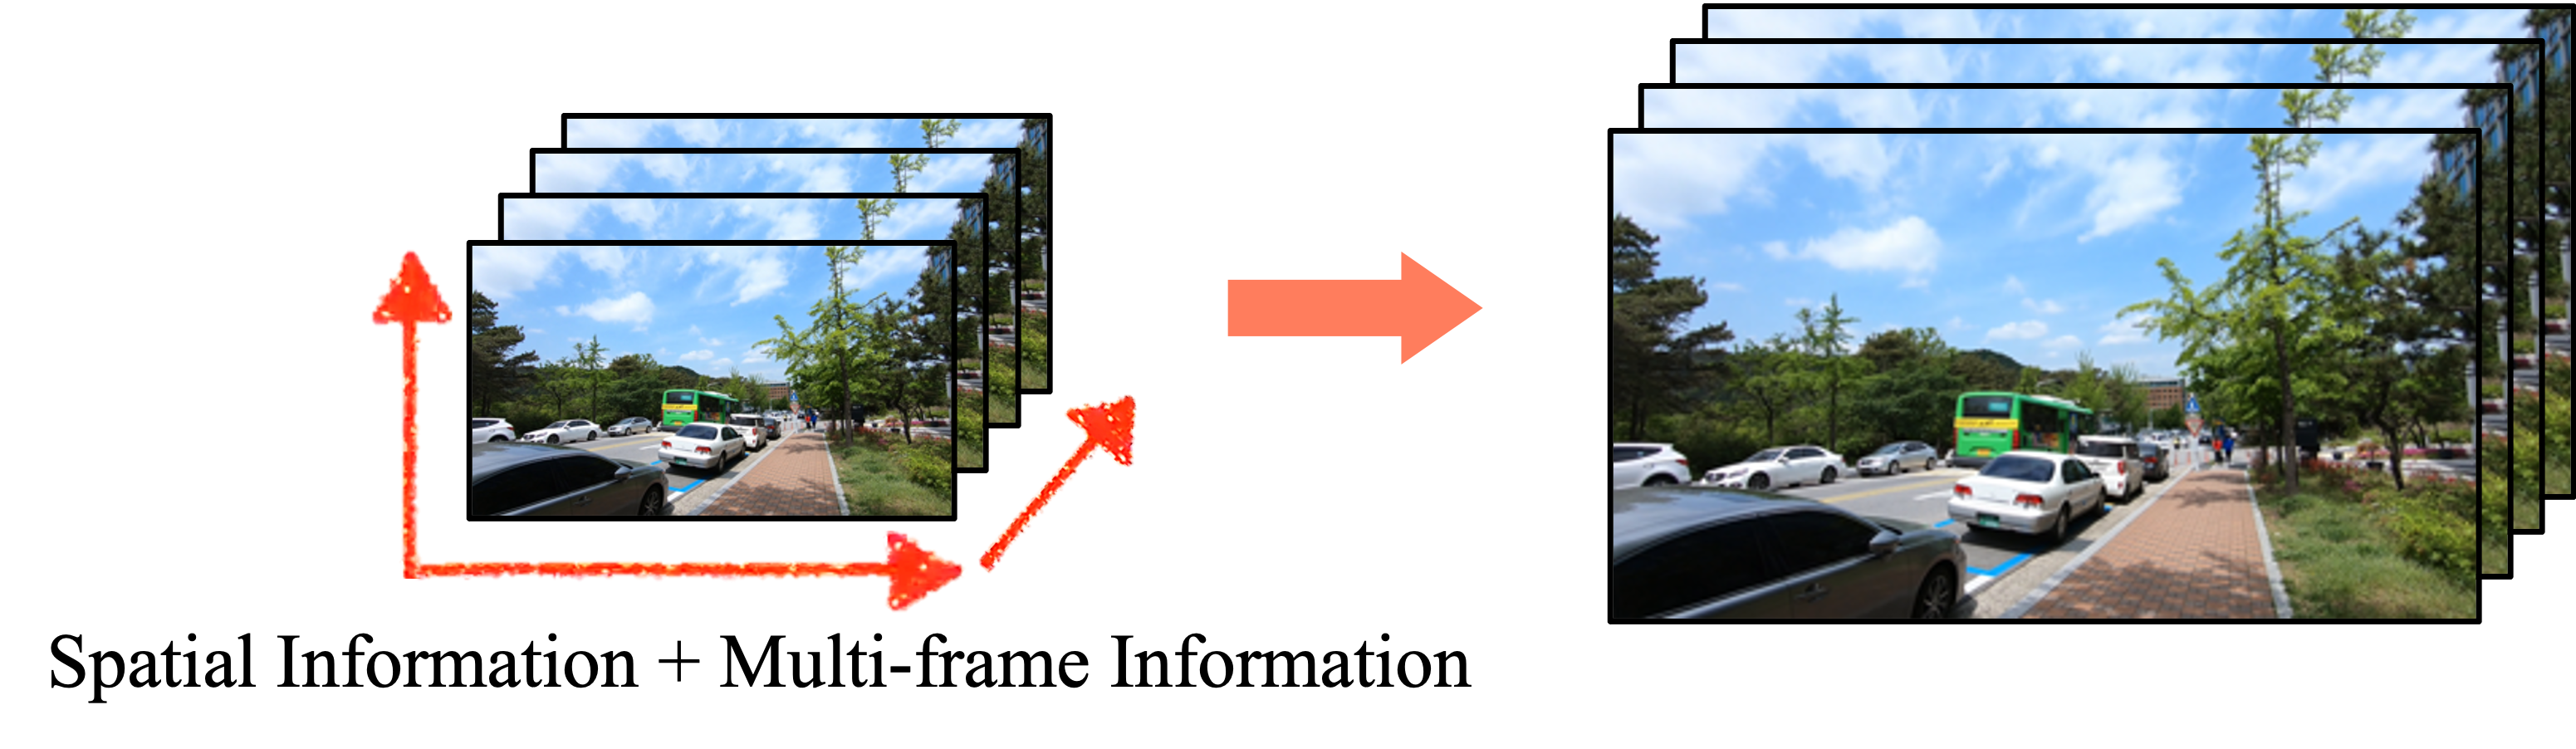
\includegraphics[width=\linewidth]{2.png}
	\caption{JPEG 基本系统压缩过程框图}
	\label{fig:fig2}
	\vspace{-0.6cm}
\end{figure}

具体来说,首先将原始图像分割成 $8\times 8$ 的子块,对于彩色图像,它要求 YUV 4:2:2格式。为消除直流电平的影响,将原始图像的所有像素减去128,再进行 DCT 变换进行去相关性。然后进行四舍五入取整,这也是图像质量下降的主要原因,JPEG 给出了量化系数矩阵表,在量化表设计时考虑了人眼的视觉特性。在编码输出时,对于直流系数预测,预测后进行熵编码;而对于交流系数,首先对交流系数进行Z型扫描,编码以游程-幅值 Huffman编码的形式完成。JPEG过程在进行分块后对每一块进行DCT变换,高压缩比时,线性量化的量化步长较大,量化后将一些高频系数变成了0,反变换后,成为了全灰的,能看到明显的方块效应。为了改善或者消除方块效应,可以用小波变化代替余弦变换,也可以降低量化步长或者在分块时 overlap,当然也可以采用后处理的方法。

正交变换一般是线性变换,其基本线性运算式严格可逆,并且满足一定的正交条件。而对于深度学习而言,更重要的是模型的非线性能力,因此直觉上来讲用深度学习的方法来做正交变换是行不通的。因此基于深度学习的正交变换主要从两个方向进行调研:基于深度学习的稀疏表示和正交变换在深度学习方法中的应用。

传统的模式识别里面,主要是对信号进行特征提取,然后对特征进行识别,这样既能减除大部分无谓的干扰,又能降低识别的运算量。提取特征最简单的方式就是正交变换,正交变换是无损的特征提取,可以在信号与特征之间互相转换。比较典型的一个应用是基于Gabor变换的纹理分析。对于纹理分析而言,采用 Gabor 滤波具有较好的时-频局部特性,它能够同时表示和捕捉二维信号在空间位置、空间频率、方向选择性和相位、频率带宽等方面的信息。用 Gabor 滤波器对图像信号滤波,相当于将其按不同方向、频段进行分解,如果计算经不同方向、频段滤波后的纹理特征,这些特征将具有明显的差异,根据这些差异就可以区分不同的纹理。正交变化具有能量集中特点,也就是能把决大部分信息集中到很小的数据量上,这个也是稀疏编码的概念。如果可以接受细微的差别,我只处理前面重要特征即可,音视频压缩也用到这个性质。

稀疏编码算法是寻找一组``超完备''\footnote{如果 $M$ 个基向量刚好可以支撑 $M$ 维的欧氏空间,则这 $M$ 个基向量是完备的。如果 $M$ 个基向量可以支撑 $D$ 维的欧氏空间,并且 $M>D$,则 这 $M$ 个基向量是过完备的(overcomplete)、冗余的。“过完备”基向量是指基向量个数远远大于其支撑空间维度。因此这些基向量一般不具备独立、正交等性质
}基向量来更高效地表示样本数据的一种无监督学习方法。稀疏编码算法的目的就是找到一组基向量 $\Phi_i$,使得我们能将输入向量 $x$ 表示为这些基向量的线性组合:

\begin{equation}
\mathbf{x}=\sum_{i=1}^k a_i \phi_i
\end{equation}

超完备基的好处是它们能更有效地找出隐含在输入数据内部的结构与模式。然而,对于超完备基来说,系数 $a_i$ 不再由输入向量 $x$ 唯一确定。

这里的“稀疏性”定义为只有很少的几个非零元素或只有很少的几个远大于零(显著不为零)的元素。要求系数 $a_i$ 是稀疏的意思就是说对于一组输入向量,我们只想有尽可能少的几个系数远大于零。选择使用具有稀疏性的分量来表示我们的输入数据是有原因的,因为绝大多数的感官数据,比如自然图像,可以被表示成少量基元素的叠加,在图像中这些基本元素可以是面或者线。

把 $m$ 个输入向量的稀疏编码代价函数定义为: 

\begin{equation}
\min _{a_i^{(j)}, \phi_i} \sum_{j=1}^m\left\|\mathbf{x}^{(j)}-\sum_{i=1}^k a_i^{(j)} \phi_i\right\|^2+\lambda \sum_{i=1}^k S\left(a_i^{(j)}\right)
\end{equation}

基向量($\Phi_i,i=1,2,…,k$)对于全部的输入向量(训练样本都是一致的),系数 $a^{(j)}_i$ 是与输入向量 $x^{(j)}$ 相对应的,由基($\Phi_i$)和输入向量($x^{(j)}$)共同决定,通过其上下标($a^{(j)}_i$)即可看出。通过最优化函数得到的 $k$ 个基向量($\Phi_i$)以及全部的输入样本在该基下的表示 $a^{(j)}_i$。此处 $S(\cdot)$ 是一个稀疏代价函数,由它来对远大于零的 $a_i$ 进行“惩罚”。稀疏编码的每一维都可以被看作一种特征。和基于稠密向量的分布式表 示相比,稀疏编码具有更小的计算量和更好的可解释性等优点。


自编码器是通过无监督的方式来学习一组数据的有效编码(或表示),自编码器的结构可分为两部分:编码器和解码器。假设有一组 $D$ 维的样本 $\boldsymbol{x}^{(n)} \in \mathbb{R}^D, 1 \leq n \leq N$, 自编码器将这组数据映射到 特征空间得到每个样本的编码 $z^{(n)} \in \mathbb{R}^M, 1 \leq n \leq N$, 并且希望这组编码可以重 构出原来的样本。这一过程有点儿类似于正交变换的正变换和逆变换,与之不同的是这一过程不是线性的,也就导致逆变换得到的结果是与原信号不同的,但其目的是要尽可能重构出原来的信号。

更进一步,如果特征空间的维度 $M$ 小于原始空间的维度 $D$,自编码器相当于是一种降 维或特征抽取方法.如果 $M \geq D$,一定可以找到一组或多组解使得 $f \circ g$ 为单位函数(Identity Function),并使得重构错误为 0。然而这样的解并没有太多的意义,但是,如果再加上一些附加的约束,就可以得到一些有意义的解,比如编码 的稀疏性、取值范围,$f$ 和 $g$ 的具体形式。

在应用方面,正交变换的作用可以分为两种,一是降低模型的计算开销,二是在频率域对图像进行特征提取和模型训练。Li \cite{DBLP:conf/ijcnn/LiYR18} 等提出采用卷积定理将空域中的卷积转换为频域中的乘积的神经网络,可用于图像超分辨率重建。该网络在测试中计算效率非常高,而且其参数通过误差反向传播来进行学习,并且由于使用Hartley变换替代傅立叶变换,因此没有复数运算。Michael等 \cite{DBLP:conf/cvpr/RamamonjisoaFWL21} 受到小波分解可以实现的稀疏表示的启发提出了一种替代网络表示,使用小波分解进行更有效的深度 估计,称之为 Wavelet-Monodepth。深度图像通常由许多分段的平坦区域组成,平坦区域之间的深度有一些“跳 跃”。这种结构非常适合小波。低频分量可以代表整个场景结构,而高频分量可以很好地捕捉“跳跃”。至关重要的是,高频分量是稀疏的,这意味着计算只能集中在某些区域。这具有节省运行时计算的效果,同时仍然能够估计高质量的深度。Zhongwei Qiu等 \cite{DBLP:conf/eccv/QiuYFF22} 提出时空-频率Transformer来解决视频压缩过程中由于分块、正交变换和量化编码产生的高频伪影对视频超分辨率重建的影响。具体来讲就是利用离散余弦变换获得图像的频谱,将原始 Transformer 中 token 的划分转变为在频谱图上的划分,从而充分利用时空-频率的相关信息来完成压缩视频的超分辨率重建。


